%%----------------------------------------------------------------------------
%% Onderzoekstechnieken: Analyse van 1 variabele
%%----------------------------------------------------------------------------

\documentclass[aspectratio=169]{beamer}

%==============================================================================
% Aanloop
%==============================================================================

%---------- Vormgeving --------------------------------------------------------

\usetheme{hogent}

\usecolortheme{hgwhite} % witte achtergrond, zwarte tekst

\usepackage{graphicx,multicol}
\usepackage{comment,enumerate,hyperref}
\usepackage{amsmath,amsfonts,amssymb}
\usepackage[dutch]{babel}
\usepackage{multirow}
\usepackage{eurosym}
\usepackage{listings}
\usepackage{textcomp}
\usepackage{framed}
\usepackage{wrapfig}
\usepackage{tabu} %needed for \tabulinesep
\usepackage{wrapfig}
\usepackage{pgf-pie}
\usepackage{pgfplots}
\usepackage{booktabs}

%---------- Configuratie ------------------------------------------------------

\pgfplotsset{compat=1.16}
\usetikzlibrary{arrows,shapes,backgrounds,positioning,shadows}
\usetikzlibrary{pgfplots.statistics}

%---------- Commando-definities -----------------------------------------------

\newcommand{\tabitem}{~~\llap{\textbullet}~~}
\newcommand{\alertbox}[2][hgblue]{%
  \setbeamercolor{alertbox}{bg=#1,fg=white}
  \begin{beamercolorbox}[sep=2pt,center]{alertbox}
    \textbf{#2}
  \end{beamercolorbox}
}

%---------- Info over de presentatie ------------------------------------------

\title{Hst 3. Analyse van 1 variabele}
\subtitle{Onderzoekstechnieken}
\author{Thomas Aelbrecht \and Jens Buysse \and Wim {De Bruyn} \and Pieter-Jan Maenhaut \and Bert {Van Vreckem}}
\date{AJ 2020--2021}

%==============================================================================
% Inhoud presentatie
%==============================================================================

\begin{document}

\begin{frame}
  \maketitle
\end{frame}

\begin{frame}
  \frametitle{What's on the menu today?}

  \tableofcontents
\end{frame}

\begin{frame}
  \frametitle{Leerdoelen}

  \begin{itemize}
    \item Beschrijvende statistiek
    \item Centrum- en spreidingsmaten voor elk meetniveau
    \item Formules kennen, kunnen uitrekenen
    \item Geschikte visualisatietechnieken voor elk meetniveau
  \end{itemize}
\end{frame}

\section{Centrum- en spreidingsmaten}

\begin{frame}
  \frametitle{Hoe groot zijn mijn vrienden?}

  Herinner je onze superhelden:

  \begin{tikzpicture}[xscale=4,yscale=2]
  \draw (0,2) -- (0,0);
  \foreach \num/\label in {0/0, 0.2/20, .4/40, .6/60, .8/80, 1/100, 1.2/120, 1.4/140, 1.6/160, 1.8/180, 2/200}{%
    \draw (0, \num) -- (2.5, \num);
    \draw[shift={(0, \num)}] (1pt,0pt) -- (-1pt,0pt) node[left] {\scriptsize \label};
  }

  \node[anchor=north] (hero1) at (0.3,1.5)
  {\includegraphics[height=2.9cm]{les2-hero-1}};
  \node[anchor=north] (hero2) at (0.8,2.05)
  {\includegraphics[height=4cm]{les2-hero-2}};
  \node[anchor=north] (hero3) at (1.3,1.575)
  {\includegraphics[height=3.1cm]{les2-hero-3}};
  \node[anchor=north] (hero4) at (1.8,2.1)
  {\includegraphics[height=4.1cm]{les2-hero-4}};
  \node[anchor=north] (hero5) at (2.3,1.95)
  {\includegraphics[height=3.8cm]{les2-hero-5}};

  \node (size1) at (0.3, 1.5) {\scriptsize 141 cm};
  \node (size2) at (0.8, 2.1) {\scriptsize 198 cm};
  \node (size3) at (1.3, 1.51) {\scriptsize 143 cm};
  \node (size4) at (1.8, 2.15) {\scriptsize 201 cm};
  \node (size5) at (2.3, 1.95) {\scriptsize 184 cm};
  \end{tikzpicture}
\end{frame}


\subsection{Centrummaten}

\begin{frame}
  \frametitle{Centrummaten}

  \Large Welke waarde is representatief voor de hele groep?
\end{frame}

\begin{frame}
  \frametitle{Gemiddelde (of \emph{mean}, \emph{average})}

  \alertbox{Het \textcolor{hgyellow}{gemiddelde} is de som van alle waarden gedeeld door het aantal waarden}

  \[ \overline{x} = \frac{1}{n} \sum_{i=1}^n x_i \]

  \input{heroes}

\end{frame}

\begin{frame}
  \frametitle{Gemiddelde (of \emph{mean}, \emph{average})}


  \vspace{.5cm}
  \begin{description}
    \item[Vraag 1] Wat gebeurt er als Kabouter Wesley (10cm) er bij komt?
    \item[Vraag 2] Het gemiddelde van 15 cijfers is 12. Welk nummer moeten we aan de rij van cijfers toevoegen om een gemiddelde van 13 te komen?
  \end{description}

  \centering \includegraphics[width=4cm]{les2-hero-6}

\end{frame}

\begin{frame}
  \frametitle{Mediaan (\emph{median})}

  \alertbox{Om de \textcolor{hgyellow}{mediaan} te vinden, sorteer de waarden en kies het middelste getal}

  \begin{itemize}
    \item Oneven aantal getallen: geen probleem
    \item Even aantal getallen: gemiddelde van de middelste twee
  \end{itemize}

  \input{heroes}

\end{frame}

\begin{frame}
  \frametitle{Mediaan (\emph{median})}

  \begin{description}
    \item[Vraag 1] Wat gebeurt er nu als Kabouter Wesley er bij komt?
    \item[Vraag 2] Gegeven het totaal aantal mensen gered door Batman de laatste 8 jaar, wat is de mediaan?
  \end{description}

  \centering
  \begin{tabular}{|c|c|c|c|c|c|c|c|}
    \hline
    4 & 7 & 11 & 16 & 20 & 22 & 25 & 26 \\
    \hline
  \end{tabular}
  \includegraphics[width=.6cm]{les2-hero-2}
\end{frame}

\begin{frame}
  \frametitle{Modus (\emph{mode})}

  \alertbox{De \textcolor{hgyellow}{modus} is het vaakst voorkomende getal in een reeks getallen}

  Totaal aantal mensen gered door Superman de laatste 15 jaar:

  \begin{center}
    \begin{tabular}{|c|c|c|c|c|c|c|c|c|c|c|c|c|c|c|}
      \hline
      3&7&5&13&20&23&39&23&40&23&14&12&56&23&29\\
      \hline
    \end{tabular}
    \includegraphics[width=.7cm]{les2-hero-3}
  \end{center}


  Totaal aantal mensen gered door Batman de laatste 8 jaar:
  \begin{center}
    \begin{tabular}{|c|c|c|c|c|c|c|c|c|}
      \hline
      4 & 7 & 11 & 16 & 20 & 22 & 25 & 26 & 33 \\
      \hline
    \end{tabular}
    \includegraphics[width=.6cm]{les2-hero-2}
  \end{center}

\end{frame}

\subsection{Spreidingsmaten}

\begin{frame}
  \frametitle{Spreidingsmaten}

  \Large Hoe groot zijn de onderlinge verschillen binnen de groep?
\end{frame}


\begin{frame}
  \frametitle{Bereik (\emph{range})}

  \alertbox{Het \textcolor{hgyellow}{bereik} van een reeks getallen is de absolute waarde van het verschil tussen het grootste en kleinste getal in de reeks.}

  \input{heroes}

\end{frame}

\begin{frame}
  \frametitle{Kwartielen (\emph{quartiles})}

  \alertbox{De \textcolor{hgyellow}{kwartielen} van een gesorteerde reeks getallen zijn de waarden die de lijst in vier gelijke delen verdeelt. Elk deel vormt dus een kwart van de dataset. Men spreekt van een eerste, tweede en derde kwartiel, genoteerd als resp,~$Q_1$, $Q_2$, $Q_3$}

  \vspace{1cm}

  Totaal aantal mensen gered door Superman de laatste 15 jaar:
  \begin{center}
    \begin{tabular}{|c|c|c|c|c|c|c|c|c|c|c|c|c|c|c|}
      \hline
      3&7&5&13&20&23&39&23&40&23&14&12&56&23&29\\
      \hline
    \end{tabular}
    \includegraphics[width=.7cm]{les2-hero-3}
  \end{center}

\end{frame}

\begin{frame}
  \frametitle{Variantie en standaardafwijking}

  Eng. \emph{variance}, resp. \emph{standard deviation}

  \bigskip

  \alertbox{De \textcolor{hgyellow}{variantie} van een steekproef ($s^2$) is de som van de gekwadrateerde verschillen tussen de waarde van de dataset en het gemiddelde, gedeeld door het aantal waarden min één}

  \[ s^2 = \frac{1}{n - 1} \sum_{i=1}^{n} (x_i - \overline{x})^2 \]


  \bigskip

  \alertbox{De \textcolor{hgyellow}{standaardafwijking} ($s$) is de vierkantswortel van de variantie}

  \input{heroes}
\end{frame}

\begin{frame}
  \frametitle{Eigenschappen standaardafwijking}

  \begin{itemize}
    \item<+-> Kan de standaardafwijking negatief zijn?
    \item<+-> Wat is de kleinst mogelijke waarde? Wat duidt dit aan?
    \item<+-> Wat is de invloed van uitschieters op de standaardafwijking?
    \item<+-> In welke eenheid staat de standaarddeviatie?
    \item<+-> Hoe interpreteer je de standaardafwijking in combinatie met het gemiddelde?
  \end{itemize}
\end{frame}

\begin{frame}
  \frametitle{Eigenschappen standaardafwijking}

  Waarom $n-1$ in de noemer en niet $n$?

  De reden voor de wijziging kan je wiskundig bewijzen, maar we gaan het empirisch onderzoeken

  \vfill

  R-script: \href{https://github.com/HoGentTIN/onderzoekstechnieken-cursus/blob/master/cursus/data/sample-variance.R}{cursus/data/sample-variance.R}
\end{frame}

\begin{frame}[plain]

  \includegraphics[width=\textwidth]{les2-01}
\end{frame}

\begin{frame}
  \frametitle{Onthou dit!}

  \alertbox{Enkel een centrummaat opgeven is nooit voldoende!}

  \begin{itemize}
    \item Wat is de spreiding?
    \item Hoe is de data verdeeld? Normale verdeling?
    \item Is de groep voldoende homogeen?
  \end{itemize}
\end{frame}

\subsection{Samenvatting}

\begin{frame}
  \frametitle{Centrum- en spreidingsmaten: samenvatting}

  \centering
  \begin{tabular}{lll}
  	\toprule
  	\textbf{Meetniveau} & \textbf{Centrummaten} & \textbf{Spreidingsmaten}      \\
  	\midrule
  	Kwalitatief         & Modus                 & ---                           \\
  	\midrule
  	Kwantitatief        & Gemiddelde            & Variantie, standaardafwijking \\
  	                    & Mediaan               & Bereik, interkwartielafstand  \\
  	\bottomrule
  \end{tabular}
\end{frame}

\begin{frame}
  \frametitle{Overzicht symbolen}

  {\tabulinesep=1.2mm
    \begin{center}
      \begin{tabular}{rcc}
      	\toprule
      	                  & \textbf{Populatie} & \textbf{Steekproef} \\
      	\midrule
      	 aantal elementen &        $N$         &         $n$         \\
      	       gemiddelde &       $\mu$        &   $\overline{x}$    \\
      	        variantie & $\sigma^2 = \frac{\sum (x_i-\mu)^2}{N}$ & $s^2  = \frac{\sum (x_i-\overline{x})^2}{n-1}$ \\
      	standaarddeviatie &      $\sigma$      &         $s$         \\
      	\bottomrule
      \end{tabular}
    \end{center}
  }
\end{frame}

\section{Grafieken}

\subsection{Eenvoudige grafieken}

\begin{frame}
  \frametitle{Cirkeldiagram (\emph{pie chart})}

  \centering
  \includegraphics[width=.8cm]{les2-hero-3}
  Waarom herkent niemand Superman?
  \begin{tikzpicture}[scale=.5]
  \pie[text=legend,color={hgblue,hgorange,hglightgreen}]{%
    3/Heeft herkend, 5/Twijfelt, 92/Lijdt aan prosopagnosia}
  \end{tikzpicture}

\end{frame}

\begin{frame}
  \frametitle{Cirkeldiagram}

  Voordelen:
  \begin{itemize}
    \item Met percentages rond 20\% kan je makkelijk verduidelijken t.o.v. volledige dataset
  \end{itemize}
  Nadelen:
  \begin{itemize}
    \item Vergelijken op basis van hoek, terwijl lengte intuïtiever is
    \item Figuur onduidelijk bij veel categorieën
  \end{itemize}
\end{frame}

\begin{frame}
  \frametitle{Cirkeldiagram}

  \begin{center}
    \alertbox{Vermijd het gebruik van cirkeldiagrammen!}

    \includegraphics[width=.6\textwidth]{pie-chart.png}
  \end{center}

\end{frame}

\begin{frame}
  \frametitle{Staafdiagram (\emph{bar chart})}

  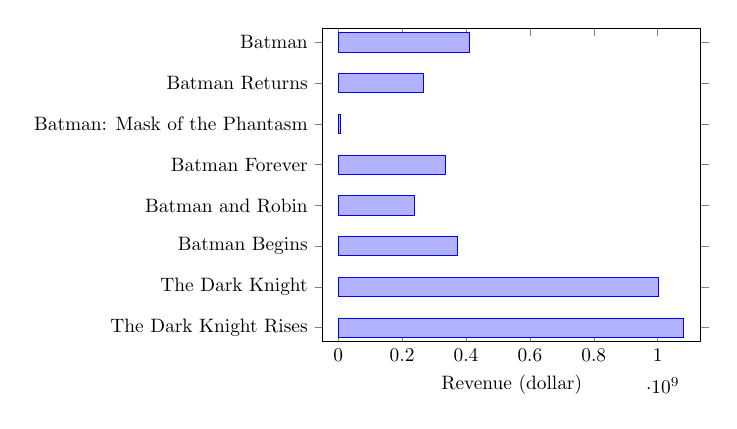
\begin{tikzpicture}[scale=.7]
  \begin{axis}[
  xbar,
  enlargelimits=0.05,
  legend style={at={(0.5,-0.2)}, anchor=north,legend columns=-1},
  ytick=data,
  symbolic y coords={The Dark Knight Rises, The Dark Knight, Batman Begins, Batman and Robin, Batman Forever, Batman: Mask of the Phantasm, Batman Returns, Batman},
  xlabel=Revenue (dollar)
  ]
  \addplot
  coordinates {
    (1080472000,The Dark Knight Rises)
    (1002000000,The Dark Knight)
    (372710000,Batman Begins)
    (238207000,Batman and Robin)
    (336529000,Batman Forever)
    (5617000,Batman: Mask of the Phantasm)
    (266822000,Batman Returns)
    (411348000,Batman)};
  \end{axis}
  \end{tikzpicture}
\end{frame}

\begin{frame}
  \frametitle{Staafdiagram}
  % Source: http://mirrors.ibiblio.org/CTAN/graphics/pgf/contrib/pgfplots/doc/pgfplots.pdf
  % p.79
  \begin{center}
    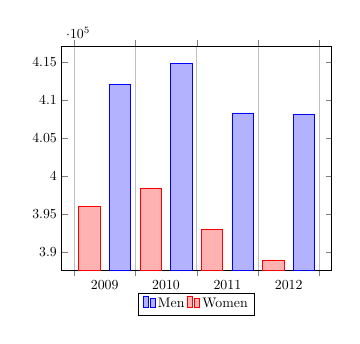
\begin{tikzpicture}[scale=.5]
    \begin{axis}[
    x tick label style={
      /pgf/number format/1000 sep=},
    xlabel=Year,
    enlargelimits=0.05,
    legend style={at={(0.5,-0.1)},
      anchor=north,legend columns=-1},
    ybar interval=0.7,
    ]
    \addplot
    coordinates {(2012,408184) (2011,408348)
      (2010,414870) (2009,412156) (2008,415 838)};
    \addplot
    coordinates {(2012,388950) (2011,393007)
      (2010,398449) (2009,395972) (2008,398866)};
    \legend{Men,Women}
    \end{axis}
    \end{tikzpicture}
  \end{center}
  Voordelen:

  \begin{itemize}
    \item Makkelijker vergelijken van categorieën
    \item Per categorie meerdere ``bars'' mogelijk
  \end{itemize}
\end{frame}


\begin{frame}
  \frametitle{Boxplot}
  \begin{columns}
    \column{.5\textwidth}
    % Source: http://mirrors.ibiblio.org/CTAN/graphics/pgf/contrib/pgfplots/doc/pgfplots.pdf
    % p.430
    \begin{tikzpicture}[scale=.9]
    \begin{axis}[x=3cm,xticklabels={},xmax=2.3]
    \addplot+[
    boxplot prepared={
      draw direction=y,
      lower whisker=5,
      lower quartile=7,
      median=8.5,
      upper quartile=9.5,
      upper whisker=10,
    },
    ]
    table[row sep=\\,y index=0] {
      data\\ 1\\ 3\\
    }
    [right,color=hgorange]
    node at
    (boxplot box cs: 1,.6)
    {uitschieter}
    node at
    (boxplot box cs: \boxplotvalue{lower quartile},1)
    {$Q_1$}
    node at
    (boxplot box cs: \boxplotvalue{median},1)
    {$Q_2$, mediaan}
    node at
    (boxplot box cs: \boxplotvalue{upper quartile},1)
    {$Q_3$}
    node at
    (boxplot box cs: \boxplotvalue{upper whisker},1)
    {max}
    ;
    \end{axis}
    \end{tikzpicture}

    \column{.5\textwidth}
    Voordeel: snelle manier om data te inspecteren en verschillende datasets te vergelijken
  \end{columns}
\end{frame}

\subsection{Interpretatie van grafieken}

\begin{frame}
  \frametitle{Data-ambiguïteit}
  \framesubtitle{= Niet aanduiden wat de data betekent.}

  \begin{columns}
    \column{.5\textwidth}
    \includegraphics[width=\textwidth]{les2-02}
    \column{.5\textwidth}
    Tips:
    \begin{itemize}
      \item Benoem je assen
      \item Geef een duidelijke titel
      \item Benoem de meeteenheid (en evt. grootorde)
      \item Voeg een bijschrift toe met uitleg over de grafiek
    \end{itemize}
  \end{columns}
\end{frame}

\begin{frame}
  \frametitle{Data distortion}
  \framesubtitle{= Verkeerde conclusies laten trekken uit een grafische voorstelling}

  \bigskip

  \begin{center}
    \includegraphics[height=.8\textheight]{les2-03}
  \end{center}
\end{frame}

\begin{frame}
  \frametitle{Data distortion}

  \begin{center}
    \includegraphics[width=.8\textwidth]{les2-03-2}
  \end{center}
\end{frame}

\begin{frame}
  \frametitle{Data distraction}

  \begin{itemize}
    \item Vermijd toeters en bellen in je grafieken
    \item Minimaliseer inkt tot data ratio
  \end{itemize}

  \centering
  \includegraphics[width=.3\textwidth]{les2-04}
  \includegraphics[width=.3\textwidth]{les2-05}

  \includegraphics[width=.3\textwidth]{les2-06}
  \includegraphics[width=.3\textwidth]{les2-07}
\end{frame}

\begin{frame}
  \frametitle{Anscombe's Quartet}

  \centering
  \includegraphics[height=.6\textheight]{anscombes_quartet}

  Vier verschillende datasets met dezelfde statistische eigenschappen. Deze tonen het belang aan van data-visualisatie.
\end{frame}

\begin{frame}[plain]
  \centering

  \includegraphics[height=.9\textheight]{1var-datasaurus-dozen.png}

  ``The datasaurus dozen'' (Bron: \url{https://www.autodeskresearch.com/publications/samestats})
\end{frame}


\end{document}
